\chapter{Yêu cầu, phạm vi và hai phiên bản}
\section{Đối chiếu với yêu cầu trên bảng}
Sản phẩm cần demo trực tiếp được, có nhánh dữ liệu/mô hình và nhánh tri thức hội tụ ở hệ đa agent; phải chỉ được KB, KG, RAG lấy từ đâu và lưu tại đâu. Tệp Cypher phải nạp lại Neo4j được. Báo cáo cần giải thích phiên bản sau khác phiên bản trước, cấu hình model và kết quả thực nghiệm, thay vì chỉ mô tả hình giao diện.

Tài liệu kiến trúc giảng viên gửi bổ sung yêu cầu về Data Agent, Prediction Agent, Rule-Based Agent, KG/RAG Agent, Coordinator, Explanation và Monitoring. Tài liệu gợi ý sáu tầng và coi RL là mở rộng tùy chọn. V2 áp dụng cấu trúc đó ở quy mô một ứng dụng local; không tự tăng số dịch vụ hoặc số agent chỉ để làm sơ đồ phức tạp.

\section{Mốc V1 và định nghĩa V2}
V1 là ứng dụng GlucoGuide đã có trước lượt nâng cấp này: FastAPI, chat Qwen4B local, KB 58 đoạn, Neo4j 169 nút/106 cạnh, hai model nghiên cứu classification/regression và bộ xuất KB/KG/RAG. Hai PDF V1 được giữ nguyên trong archive, không ghi đè.

V2 bổ sung mục \emph{Thực nghiệm V1/V2}, API nghiên cứu riêng, hai bộ dữ liệu nhị phân và quy trình điều phối có mã lượt chạy. V1 đối chứng trong mục mới là cấu hình 64--32--16 được huấn luyện lại trên Pima và Early Stage. V2 thêm hai lớp 8 và 4 neuron, đổi L2 và cân bằng trọng số lớp. Mỗi bộ có checkpoint riêng cho hai cấu hình. Giữ nguyên dataset và mẫu khi đổi phiên bản để đối chiếu kết quả.
\par\FloatBarrier\begin{table}[H]\centering\small\setstretch{1.15}\setlength{\tabcolsep}{5pt}
\caption{V1 và phần nâng cấp V2 có thể kiểm tra.}\begin{tabular}{P{2.6cm}P{5.6cm}P{5.6cm}}\toprule
Hạng mục & V1 gốc / đối chứng & V2\\\midrule
Dữ liệu model & 50K nhãn tổng hợp và hồi quy; giữ nguyên checkpoint gốc. & Thêm Pima và Early Stage nhị phân; kiểm kê trùng và nguồn.\\
Mạng đối chứng & Ba tầng ẩn 64--32--16. & Năm tầng ẩn 64--32--16--8--4, L2 mạnh hơn và trọng số lớp cân bằng.\\
MAS & Có MessageBus và các handler chuyên trách. & Thêm workflow riêng sáu tầng, bảy vai trò, schema theo dataset.\\
Truy vết & Trace sender/receiver/type/content trong response. & Thêm request ID, version, status, timing, hash và audit metadata.\\
KB / KG / chat & 58 đoạn, 169 nút, 106 cạnh, TF-IDF và Qwen4B. & Tái sử dụng nguyên; không nhận là các thành phần mới hoặc fine-tune mới.\\
Tài liệu nộp & Tiểu luận Final, Project 01 và các tệp thực nghiệm. & Tiểu luận phát triển từ Final, Project 01, Cypher, ZIP và hướng dẫn.\\\bottomrule\end{tabular}\end{table}


\section{Những chức năng từ Project 01 gốc được dùng lại}
Mục \emph{Phân loại \& dự đoán} vẫn phục vụ hai bài toán gốc. Mô hình phân loại trả High, Moderate, Low trên nhãn tổng hợp. Mô hình hồi quy trả điểm tiến triển nghiên cứu sau một năm. Người dùng có thể chuyển kết quả sang luồng nhận xét và hỗ trợ có nguồn. Hai mô hình được nạp tại \code{app/main.py}, dòng 29--30, và gọi qua \code{/api/chat} khi người dùng chọn tác vụ dữ liệu.

Kết quả lưu của bản gốc gồm accuracy 0,818 và macro-F1 0,5441 cho MLP phân loại trên 10.000 hàng test. MLP hồi quy có MAE 44,32 trên 89 hàng test. Các số đo này có nhãn, đơn vị và quần thể riêng. Bảng so sánh V1/V2 ở Chương~\ref{pr:model} dùng Pima và Early Stage theo giao thức mới.

V2 dùng lại Neo4j, bộ truy xuất và bước kiểm tra an toàn trong luồng thực nghiệm. Qwen local tiếp tục phục vụ luồng Trò chuyện. Màn hình mới cho xem cùng lúc cấu hình mạng, đoạn tri thức và mã lượt chạy. Tiểu luận Final V2 giải thích nền tảng học và cách đánh giá. Project 01 V2 đi sâu vào đường đi của yêu cầu, triển khai, kiểm thử và thao tác demo.

\section{Điều kiện chấp nhận}
Một mẫu hợp lệ phải cho kết quả từ checkpoint thật, cờ phạm vi, nguồn và trace có request ID. Một mẫu sai dừng trước model. Tình huống ưu tiên an toàn không chờ model hoặc graph. Mất Neo4j phải thể hiện trạng thái rõ, không giả dữ liệu. Bộ nộp có hai báo cáo, thư mục \code{KB_KG_RAG/} chứa Cypher và các tệp tri thức, thư mục mã nguồn và hướng dẫn.

Chương~\ref{pr:walkthrough} minh họa các lượt chạy trên giao diện. Các chương kỹ thuật tiếp theo đi sâu vào phép chia và model, cách xử lý lỗi, truy vết tài liệu, hội thoại và tái lập. Phụ lục~\ref{ch:v2-core-code} đưa các đoạn code có số dòng để đối chiếu thiết kế với chương trình đang dùng.

\Needspace{18\baselineskip}
\section{Ma trận yêu cầu và bằng chứng}
Bảng sau đối chiếu các điểm trong tài liệu kiến trúc \cite{architecture} và yêu cầu demo trên bảng với thành phần có thể mở tại bàn. Đề xuất RL của giảng viên thuộc giai đoạn mô phỏng tùy chọn. Phần thực nghiệm V2 tập trung vào model, tri thức, phối hợp và kiểm thử.
\par\FloatBarrier\begin{table}[H]\centering\small\setstretch{1.15}\setlength{\tabcolsep}{5pt}
\caption{Yêu cầu và bằng chứng có thể mở trong buổi demo.}\begin{tabular}{P{3.7cm}P{6.0cm}P{4.1cm}}\toprule
Yêu cầu & Cách thể hiện trong GlucoGuide & Mở để kiểm tra\\\midrule
Hai phiên bản và hai bộ train & V1 đối chứng và V2 dùng cùng phép chia trong mỗi bộ. V2 có năm tầng ẩn. & Chương~\ref{pr:model}, bảng test, màn V1/V2.\\
DL có thể dùng lại & Mô hình V1 gốc phục vụ luồng cũ. Nhánh V2 nạp pipeline đã huấn luyện khi suy luận. & \code{app/main.py}, \code{app/v2.py}.\\
Sáu tầng và hợp đồng agent & Coordinator gọi Data, Prediction, Rule, KG/RAG, Explanation và Monitoring. & Chương~\ref{pr:mas}, trace có mã yêu cầu.\\
Neo4j, Cypher và nguồn RAG & Nạp cạnh từ Cypher. Đối chiếu mã tài liệu, trích đoạn và URL giữa KB, đồ thị và câu trả lời. & Chương~\ref{pr:knowledge}, Neo4j Browser.\\
Đánh giá từng phần và toàn hệ & Đối chiếu checkpoint, replay retrieval, chạy API và giao diện. Tách đánh giá kỹ thuật khỏi đánh giá lâm sàng. & Chương~\ref{pr:checks}, JSON kiểm thử.\\\bottomrule\end{tabular}\end{table}


\chapter{Kiến trúc sáu tầng và phối hợp agent}\label{pr:mas}
\section{Phân tầng hệ thống}
\begin{figure}[H]\centering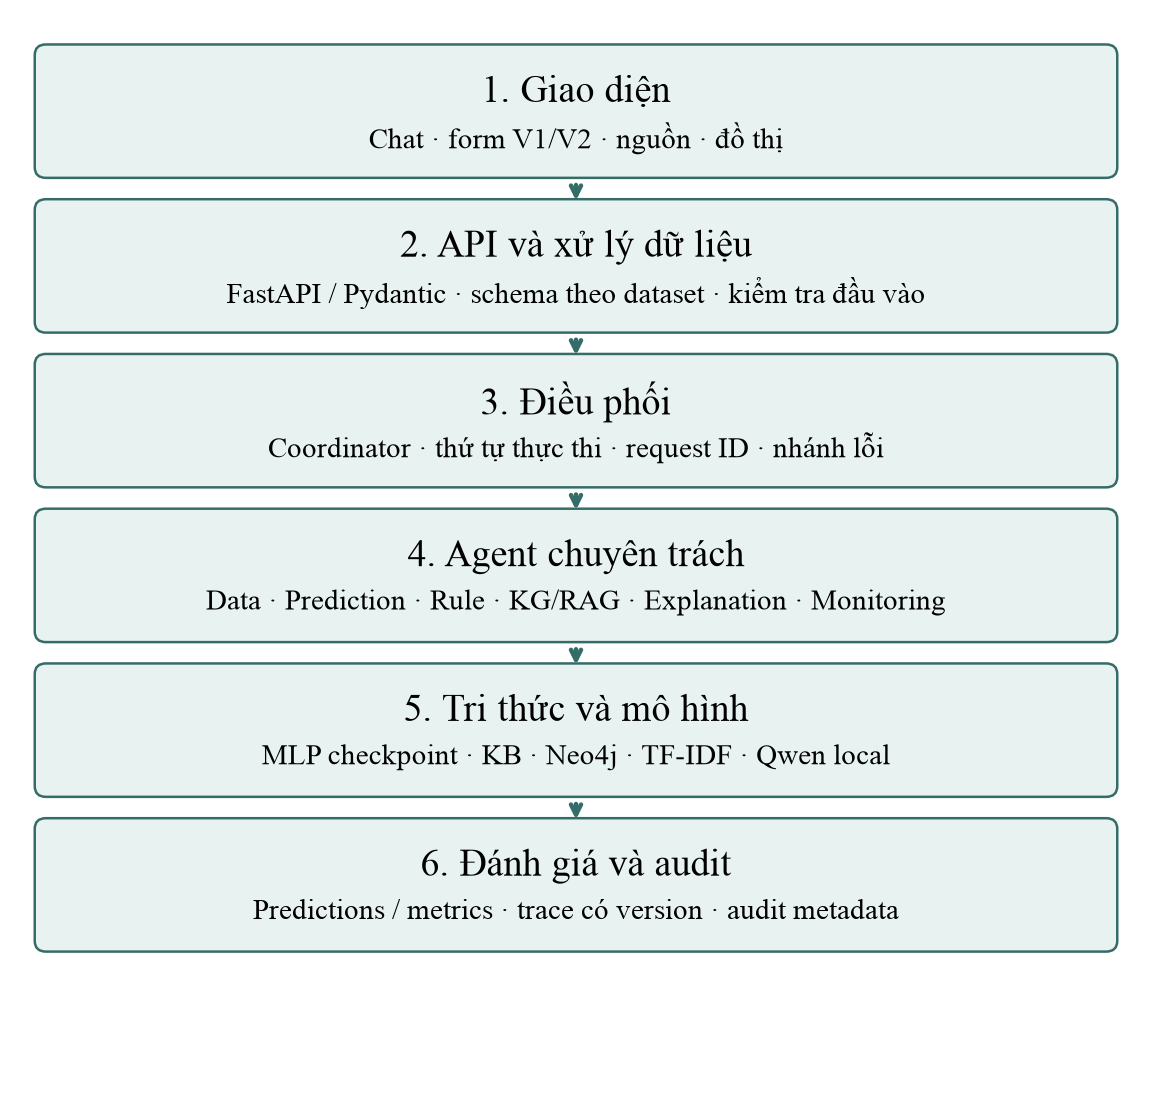
\includegraphics[width=0.78\linewidth]{figures/layers.png}\caption{Sáu tầng triển khai V2 theo đề cương của giảng viên. Backend thực hiện điều phối tập trung.}\end{figure}
Tầng 1 là web form, hội thoại, so sánh và đồ thị. Tầng 2 là FastAPI/Pydantic cùng Data Agent kiểm tra kiểu, thiếu, mã và miền quan sát. Tầng 3 là Coordinator điều khiển thứ tự và nhánh lỗi. Tầng 4 là các vai trò Data, Prediction, Rule, KG/RAG, Explanation, Monitoring. Tầng 5 là checkpoint, KB, Neo4j, chỉ mục TF-IDF và Qwen. Tầng 6 là metric, predictions, trace và audit.

Một vai trò có thể chạm nhiều tầng: Data vừa liên quan API vừa là chuyên trách kiểm tra; Monitoring là agent ghi audit nhưng bằng chứng được trình bày ở tầng đánh giá. Đây là phân tầng trách nhiệm, không phải sơ đồ lớp kế thừa hoặc sáu tiến trình mạng.

\section{Bảy vai trò và hợp đồng}
\par\FloatBarrier\begin{table}[H]\centering\small\setstretch{1.15}\setlength{\tabcolsep}{5pt}
\caption{Bảy vai trò: Coordinator điều phối sáu agent chuyên trách.}\begin{tabular}{P{2.2cm}P{4.1cm}P{4.1cm}P{3.1cm}}\toprule
Vai trò & Đầu vào & Đầu ra & Thực hiện\\\midrule
Coordinator & Request + dataset/version & Response tích hợp hoặc lỗi & Workflow trong v2.py\\
Data & Feature thô và schema & Feature order, missing flags hoặc lỗi & validate\_data\\
Prediction & Dữ liệu chuẩn hóa & Label, score, threshold, version, hash & predict / pipeline\\
Rule & Dataset, cờ dữ liệu & Cờ phạm vi và giới hạn & reviewed\_rules\\
KG/RAG & Câu hỏi kiến thức & Đoạn có nguồn, cạnh đã đối chiếu & Retriever + GraphKnowledgeAgent\\
Explanation & Model + rules + evidence & Giải thích có nguồn, không chẩn đoán & explain\\
Monitoring & Metadata lượt chạy & Trạng thái lưu request/version & monitor / JSONL\\\bottomrule\end{tabular}\end{table}

Coordinator gọi các vai trò qua MessageBus. Các lớp/handler trong \code{app/v2.py} có đầu vào và đầu ra rõ; chúng có thể kiểm thử độc lập và bị ràng buộc bởi workflow. Hệ thống chưa có thương lượng ngang hàng hay planner tự tạo nhiệm vụ tùy ý, vì vậy cần mô tả đúng là MAS điều phối tập trung với mức tự chủ giới hạn.

\section{Đường đi từ nút Chạy đến checkpoint}
Khi mở màn thực nghiệm, \code{web/v2.js}, dòng 21--29, lấy schema và cấu hình mạng từ \code{GET /api/v2/study}. Dòng 9 điền mẫu công khai từ registry. Dòng 11--16 chuyển form thành JSON, gửi \code{POST /api/v2/predict} và hiển thị nhãn, số lớp, nguồn và trace. Hai dataset có danh sách trường riêng. Khi đổi dataset, giao diện dựng lại form theo registry mới.

Tại backend, \code{app/v2.py}, dòng 63--87, kiểm tên trường, thứ tự và giá trị. Dòng 90--99 dùng pipeline từ file joblib, chọn cột xác suất của lớp 1 qua \code{classes_} và áp ngưỡng 0,5. Dòng 171 gọi Prediction qua bus. Dòng 172--177 chuyển dữ liệu và dự đoán cho Rule, rồi dừng nếu kết quả thiếu nhất quán. Dòng 187 đưa dự đoán, cờ luật và nguồn cho Explanation. Dòng 189--196 ghi metadata và trả phản hồi. Hash trong kết quả nhận diện checkpoint đã chạy, giúp đối chiếu trực tiếp với tệp thực nghiệm.

\section{Luồng thực thi và ưu tiên}
\begin{enumerate}
\item API nhận dataset, model version, features và câu hỏi kiến thức; sinh request ID.
\item Kiểm tra an toàn trước khi gọi model. Nếu ưu tiên, trả nhánh an toàn và ghi audit việc bỏ qua model.
\item Data đối chiếu schema riêng; thiếu key, NaN dạng số hoặc trường lạ bị từ chối. Null từng trường có thể được impute; thiếu toàn bộ bị từ chối.
\item Prediction nạp pipeline cố định thứ tự feature, trả nhãn, điểm, cấu hình và hash checkpoint.
\item Rule nhận dữ liệu đã kiểm tra và kết quả Prediction theo mục 6.3 của tài liệu giảng viên. Agent kiểm điểm, ngưỡng và nhãn, đồng thời ghi cờ phạm vi, quần thể và điền thiếu. Nếu đầu ra sai, API trả 503 trước Explanation.
\item KG/RAG truy xuất văn bản, lấy cạnh Neo4j và đối chiếu căn cứ. Coordinator chuyển kết quả sang Explanation.
\item Explanation trả báo cáo có nguồn. Monitoring lưu metadata; response mang trace và trạng thái lưu.
\end{enumerate}
Nhánh model V2 dùng mẫu giải thích xác định để giữ rõ phạm vi. Qwen vẫn phục vụ luồng hỏi đáp thông thường của sản phẩm. Không nên nói mọi response V2 đều được Qwen sinh, hoặc mọi agent đều là LLM.

\section{Message và audit}
Message giữ sender, receiver, type, content và thêm request ID, system version 2.0, agent version, model version, status, elapsed time. Model version có dạng \code{pima-v2-seed254}. Cả message đi và về đều gắn cùng request ID. Trạng thái requested/ok/error giúp đọc luồng và phân biệt lỗi chủ động với dữ liệu rỗng.

Trên Mac, audit được lưu tại \code{.runtime/audit-v2.jsonl}, chỉ chứa request/version, hash model, dataset, thời gian, ID nguồn, trạng thái đồ thị và kết quả kiểm tra nhất quán. Không ghi raw features, câu hỏi, câu trả lời hoặc credential vào audit này. Trace trả trong response chứa chi tiết phục vụ demo, khác bản audit đã giảm dữ liệu.

\section{Hợp đồng yêu cầu và kết quả thực tế}
\code{POST /api/v2/predict} nhận \code{dataset}, \code{version}, \code{values} và câu hỏi tùy chọn. Dataset chọn tập trường và checkpoint. Trong \code{values}, khóa thiếu hoặc lạ gây lỗi 422 ở Data Agent. Một khóa hợp lệ mang \code{null} là trường thiếu có thể điền trung vị, miễn là còn ít nhất một trường có giá trị. Điểm dự đoán, cờ luật, nguồn văn bản và cạnh đồ thị nằm ở các trường riêng để người xem đối chiếu.

Ví dụ dưới đây rút từ lượt kiểm thử Pima V2 đã lưu. Phần dự đoán chỉ ra điểm lớp Positive và ngưỡng sử dụng. Mã tài liệu \code{a1c} thuộc nhánh tri thức. Chúng đi cùng một phản hồi vì cùng lượt chạy, còn điểm mô hình được tính từ vector Pima.
\Needspace{16\baselineskip}\noindent\textbf{Yêu cầu dùng mẫu Pima công khai.}\par
\begin{Verbatim}[fontsize=\small]
{
  "dataset": "pima",
  "version": "v2",
  "values": {
    "preg": 5.0,
    "plas": 128.0,
    "pres": 80.0,
    "skin": null,
    "insu": null,
    "mass": 34.6,
    "pedi": 0.144,
    "age": 45.0
  },
  "question": "HbA1c là gì?"
}
\end{Verbatim}
\Needspace{13\baselineskip}\noindent\textbf{Trích phản hồi của lượt kiểm thử.}\par
\begin{Verbatim}[fontsize=\small]
{
  "request_id": "cd7e56596067410d932aba735ae8b274",
  "prediction": {
    "model_version": "pima-v2-seed254",
    "hidden_layers": [64, 32, 16, 8, 4],
    "label_text": "Positive",
    "positive_label_score": 0.5472,
    "threshold": 0.5
  },
  "source_ids": ["a1c"],
  "graph_status": "Neo4j"
}
\end{Verbatim}


Trace trả về trình duyệt có thể chứa nội dung yêu cầu. Audit JSONL lưu mã lượt, phiên bản, thời gian, mã nguồn và tình trạng graph. Hai dạng dữ liệu này có phạm vi khác nhau. Khi minh họa, dùng mẫu công khai trên giao diện.

\chapter{Hai dataset và huấn luyện mô hình}\label{pr:model}
\section{Nguồn, làm sạch và phép chia}
\par\FloatBarrier\begin{table}[H]\centering\small\setstretch{1.15}\setlength{\tabcolsep}{5pt}
\caption{Hai bộ dữ liệu và phép chia thực tế sau làm sạch.}\begin{tabular}{P{4.2cm}rr}\toprule
Hạng mục & Pima & Early Stage\\\midrule
Nguồn & OpenML 37 v1 & UCI 529\\
Số dòng gốc & 768 & 520\\
Sau loại trùng & 768 & 251\\
Số feature & 8 & 16\\
Train / validation / test & 460 / 154 / 154 & 150 / 50 / 51\\
Negative / Positive (sạch) & 500 / 268 & 78 / 173\\
Nhóm feature mâu thuẫn & 0 & 0\\\bottomrule\end{tabular}\end{table}

Pima là dữ liệu lịch sử có hạn chế về quần thể; Early Stage là bảng hỏi bệnh viện tại Bangladesh. Hai task đều nhị phân nhưng khác feature, label collection và population. Các khoảng min/max ở form chỉ là miền quan sát dataset, không phải ngưỡng y khoa an toàn.

Làm sạch Early Stage trước khi chia loại 269 dòng lặp, còn 251 mẫu. Pima không mất dòng trùng. Các nhóm trùng feature mâu thuẫn nhãn được kiểm kê và loại toàn bộ nếu có; snapshot này không có nhóm đó. Vì thiếu ID bệnh nhân, đây không thay cho group split theo người. Pima coi 0 ở năm phép đo là thiếu, giữ 0 mang thai hợp lệ; imputer/scaler chỉ fit train.
\sourcefile{data/v2/*.csv; models/v2/registry.json}
\par\FloatBarrier\begin{table}[H]\centering\small\setstretch{1.15}\setlength{\tabcolsep}{5pt}
\caption{Tám feature Pima; đơn vị theo mô tả nguồn, không phải ngưỡng chẩn đoán.}\begin{tabular}{P{2.2cm}P{6.5cm}P{5cm}}\toprule
Mã & Ý nghĩa & Đơn vị / xử lý\\\midrule
preg & Số lần mang thai & Số lần; 0 hợp lệ\\
plas & Plasma glucose sau 2 giờ OGTT & mg/dL; 0 coi là thiếu\\
pres & Huyết áp tâm trương & mmHg; 0 coi là thiếu\\
skin & Nếp gấp da cơ tam đầu & mm; 0 coi là thiếu\\
insu & Insulin huyết thanh sau 2 giờ & $\mu$U/mL; 0 coi là thiếu\\
mass & Chỉ số BMI & kg/m$^2$; 0 coi là thiếu\\
pedi & Diabetes pedigree function & Điểm chỉ số của dataset\\
age & Tuổi & Năm; quần thể từ 21 tuổi\\\bottomrule\end{tabular}\end{table}

Early Stage gồm Age, Gender và 14 mã Yes/No: Polyuria, Polydipsia, sudden weight loss, weakness, Polyphagia, Genital thrush, visual blurring, Itching, Irritability, delayed healing, partial paresis, muscle stiffness, Alopecia, Obesity. Từ điển theo đúng thứ tự nằm trong registry; không đổi nghĩa trường để dùng chung với Pima.

\section{Kiến trúc và điều kiện train}
V1 đối chứng có ba tầng ẩn 64--32--16. V2 thêm hai tầng 8 và 4 neuron, thành năm tầng ẩn 64--32--16--8--4. Số này đếm riêng phần giữa đầu vào và đầu ra. Cả hai dùng ReLU ở tầng ẩn và sigmoid ở đầu ra. V2 tăng L2 từ $10^{-4}$ lên $10^{-2}$ và cân bằng trọng số lớp trên tập train.

Adam learning rate $10^{-3}$, batch tối đa 32, tối đa 600 epoch và patience 60. Epoch được chọn bằng validation macro-F1, tie-break bằng validation log loss. Threshold cố định 0,5; không chọn threshold/seed theo test. Ba seed khởi tạo dùng cùng split 254; checkpoint demo chọn seed 254 từ trước. Các model train bằng scikit-learn CPU trên Mac; Qwen4B không fine-tune.
\fig{figures/mlp.png}{0.95}{Năm tầng ẩn của V2, từ 64 xuống 4 neuron trước đầu ra.}

\section{Kết quả và đánh đổi}
\par\FloatBarrier\begin{table}[H]\centering\small\setstretch{1.15}\setlength{\tabcolsep}{5pt}
\caption{Metric test; trung bình $\pm$ độ lệch chuẩn khởi tạo, không phải khoảng tin cậy.}\begin{tabular}{llrrrl}\toprule
Dataset & Mạng & Accuracy & Macro-F1 & Recall + & Tham số\\\midrule
Pima & Logistic & 0.773 & 0.734 & 0.566 & --\\
Pima & V1 & 0.762 $\pm$ 0.008 & 0.736 $\pm$ 0.008 & 0.654 $\pm$ 0.009 & 3201\\
Pima & V2 & 0.712 $\pm$ 0.026 & 0.698 $\pm$ 0.028 & 0.723 $\pm$ 0.044 & 3361\\
Early Stage & Logistic & 0.980 & 0.977 & 1.000 & --\\
Early Stage & V1 & 0.876 $\pm$ 0.033 & 0.837 $\pm$ 0.047 & 0.990 $\pm$ 0.013 & 3713\\
Early Stage & V2 & 0.922 $\pm$ 0.016 & 0.903 $\pm$ 0.025 & 0.971 $\pm$ 0.040 & 3873\\\bottomrule\end{tabular}\end{table}

\fig{figures/two_datasets.png}{1}{So sánh test theo từng dataset; không dùng chênh lệch giữa hai dataset để kết luận năng lực tổng quát.}
Ở seed demo 254, Pima có accuracy V1/V2 là 0.7532/0.7338, macro-F1 0.7267/0.7210, recall Positive 0.6415/0.7547. Chênh lệch accuracy ghép cặp V2 trừ V1 là -0.0195, khoảng bootstrap 95\% [-0.0779, 0.0325]. Logistic đối chứng đạt macro-F1 0.7336.

Ở seed demo 254, Early Stage có accuracy V1/V2 là 0.8627/0.9020, macro-F1 0.8145/0.8741, recall Positive 1.0000/1.0000. Chênh lệch accuracy ghép cặp V2 trừ V1 là 0.0392, khoảng bootstrap 95\% [0.0000, 0.0980]. Logistic đối chứng đạt macro-F1 0.9768.

Trung bình ba seed, V2 tăng macro-F1 trên Early Stage. Trên Pima, recall Positive tăng và macro-F1 giảm. Hai khoảng bootstrap đều chứa 0. Độ sâu, L2 và trọng số lớp thay đổi cùng lúc. Hai tập test đã được dùng trước đó. Cần dữ liệu mới để xác nhận.

\par\FloatBarrier\begin{table}[H]\centering\small\setstretch{1.15}\setlength{\tabcolsep}{5pt}
\caption{Ma trận nhầm lẫn ở seed demo 254; lớp Positive là lớp 1.}\begin{tabular}{llrrrr}\toprule
Dataset & Mạng & TN & FP & FN & TP\\\midrule
Pima & V1 & 82 & 19 & 19 & 34\\
Pima & V2 & 73 & 28 & 13 & 40\\
Early Stage & V1 & 9 & 7 & 0 & 35\\
Early Stage & V2 & 11 & 5 & 0 & 35\\\bottomrule\end{tabular}\end{table}

Ở seed 254, Pima V2 giảm số mẫu dương tính bị bỏ sót từ 19 xuống 13, đồng thời tăng số báo dương tính nhầm từ 19 lên 28. Trên Early Stage, số báo dương tính nhầm giảm từ 7 xuống 5 và cả hai cấu hình nhận ra đủ 35 mẫu dương tính.

\section{So từng hàng để thấy V2 sửa được lỗi nào}
\par\FloatBarrier\begin{table}[H]\centering\small\setstretch{1.15}\setlength{\tabcolsep}{5pt}
\caption{Thay đổi dự đoán trên cùng hàng test, seed 254, thứ tự V1 tới V2.}\begin{tabular}{llrrrrr}\toprule
Bộ dữ liệu & Nhãn thật & Đúng/đúng & Đúng/sai & Sai/đúng & Sai/sai & Tổng\\\midrule
Pima & Negative & 72 & 10 & 1 & 18 & 101\\
Pima & Positive & 33 & 1 & 7 & 12 & 53\\
Early Stage & Negative & 9 & 0 & 2 & 5 & 16\\
Early Stage & Positive & 35 & 0 & 0 & 0 & 35\\\bottomrule\end{tabular}\end{table}

Trên Pima, trong 53 mẫu dương tính, V2 sửa được bảy lỗi của V1 và làm sai một mẫu V1 từng đoán đúng. Trong 101 mẫu âm tính, V2 sửa một lỗi và phát sinh mười lỗi. Như vậy V2 thêm sáu dự đoán dương tính đúng nhưng giảm chín dự đoán âm tính đúng. Trên Early Stage, hai mẫu âm tính đổi từ sai sang đúng, còn toàn bộ 35 mẫu dương tính vẫn được nhận ra ở seed này.

Bảng được lập từ cùng một chỉ số hàng trong hai CSV test, dùng đúng ngưỡng 0,5. Nó bổ sung cho ma trận nhầm lẫn bằng cách chỉ ra có bao nhiêu mẫu thật sự đổi trạng thái. Ba seed sử dụng chung phép chia. Kiến trúc, L2 và trọng số lớp thay đổi đồng thời, vì vậy kết quả phản ánh cả cấu hình V2. Một thực nghiệm tách thành phần mới cho biết riêng hai lớp thêm vào đóng góp bao nhiêu.

\section{Tái lập và truy vết checkpoint}
Chạy \code{scripts/train_v2.py} để làm sạch, chia, fit và lưu. Cấu hình, hash, seed, epoch và metric nằm trong \code{results/v2/experiment.json}; các CSV cùng thư mục lưu đường học và từng dự đoán test. Checkpoint/registry nằm trong \code{models/v2/}.

Checkpoint demo seed 254 không refit; xác suất khớp CSV tới $10^{-12}$. Refit cần version, manifest và metric mới.

\chapter{KB, KG, Cypher và RAG có nguồn}\label{pr:knowledge}
\section{Ba loại dữ liệu cần phân biệt}
Dữ liệu train chứa feature và nhãn để học trọng số. KB chứa văn bản tri thức có nguồn. KG chứa khái niệm/quan hệ để truy vấn. RAG dùng index và pipeline truy xuất để cấp context cho giải thích; nạp KG không tự train MLP hay Qwen. Hai nhánh này chỉ hội tụ ở Coordinator/Explanation.
\fig{figures/provenance.png}{1}{Tách nhánh huấn luyện với nhánh tri thức, sau đó hội tụ ở workflow đa agent.}

\section{Tệp nộp và nguồn hình thành}
KB hợp nhất từ ba tệp trong data/:
\begin{itemize}
\item \code{knowledge.json}: tri thức nền.
\item \code{knowledge_dialogue.json}: đoạn phục vụ hội thoại.
\item \code{knowledge_curated.json}: nguồn web/PDF đã biên soạn, đối chiếu.
\end{itemize}
Kho có \textbf{58 đoạn từ 22 nguồn đang được sử dụng}, gồm \textbf{21 link web và 1 PDF}. Mỗi nguồn được ít nhất một đoạn tham chiếu và chỉ được đếm một lần theo URL. Mục \code{sources} trong \href{https://github.com/jellalaz/He_Thong_Thong_Minh_Thay_Que/blob/main/exports/KB_KG_RAG/KB_knowledge.json}{KB\_knowledge.json trên GitHub} liệt kê đủ 22 nguồn.

Nhóm nguồn dùng để minh họa tiêu chí trên bảng gồm ba bài web (NIDDK về sống khỏe, Vinmec về dinh dưỡng và Vinmec về chăm sóc bàn chân) cùng một PDF NIDDK \emph{Guiding Principles}. Bốn nguồn này đóng góp 12 đoạn biên soạn trong kho. Mở \nolinkurl{data/source_curation.json} để xem URL, mã đoạn và vị trí trích. PDF có số trang vật lý, còn hai bài Vinmec lưu trích dẫn ngắn và URL.

KG xuất 169 Concept và 106 RELATED\_TO, có thuộc tính nhãn quan hệ, document, evidence, URL và provenance nếu có. Tệp \code{kb_diabet.cypher} nằm trong \nolinkurl{exports/KB_KG_RAG/} trên GitHub; Nội dung trùng tệp gốc trong \nolinkurl{exports/diabetes/kg/import.cypher}. Tên \code{DB_diabet.cypher} trong tài liệu thầy là tên ví dụ, không phải một loại tệp khác.
\par\FloatBarrier\begin{table}[H]\centering\small\setstretch{1.15}\setlength{\tabcolsep}{5pt}
\caption{Năm bộ ba thật từ KB đang nạp, kèm mã tài liệu đối chiếu.}\begin{tabular}{P{3.4cm}P{3.2cm}P{3.7cm}P{3cm}}\toprule
Chủ thể & Quan hệ & Đối tượng & Document\\\midrule
HbA1c & phản ánh & đường huyết trung bình & \code{a1c}\\
Glucose & cần có & đơn vị và thời điểm đo & \code{testing}\\
Tiểu đường & liên quan đến & thiếu hoặc sử dụng insulin kém hiệu quả & \code{overview}\\
Vận động & hỗ trợ & quản lý đường huyết & \code{activity}\\
Liều thuốc & cần được chỉ định bởi & nhân viên y tế & \code{medicine}\\\bottomrule\end{tabular}\end{table}


\section{Trình diễn Neo4j}
Trong Neo4j Browser, chạy \code{CREATE CONSTRAINT} trước rồi chạy khối \code{UNWIND} và \code{MERGE} của tệp Cypher. Ràng buộc giữ tên \code{Concept} duy nhất. Chạy lại cùng tệp giữ nguyên 169 nút và 106 cạnh thuộc bộ xuất. Truy vấn đối chiếu:
\begin{quote}\small\ttfamily
MATCH (a:Concept)-[r:RELATED\_TO]->(b:Concept)\\
RETURN a, r, b LIMIT 100;\\[4pt]
MATCH (a:Concept)-[r:RELATED\_TO]->(b:Concept)\\
WHERE r.document = 'a1c'\\
RETURN a.name, r.label, b.name, r.evidence, r.source\_url;
\end{quote}
Web có nút xem toàn bộ graph và lọc 58 tài liệu. Đồ thị có 63 cụm rời; không bịa cạnh để nối các cụm. Agent lấy cạnh bằng tham số document IDs sau retrieval và kiểm tra bộ ba/văn bản/nguồn. Chưa có lập kế hoạch Cypher tự do, tìm đường đa bước hoặc xây ontology bệnh nhân.

\section{Pipeline retrieval và generation}
Chế độ truy xuất xếp hạng dùng TF-IDF từ 1--2 gram và ký tự 3--5 gram, trọng số 0,55/0,45, ngưỡng tối thiểu 0,15 và ngưỡng tương đối 0,58. Nó trả tối đa bốn đoạn. Nhánh định tuyến có nguồn cố định lấy các mã đã chỉ định. KG Agent nhận tối đa bốn mã trong cả hai trường hợp. Web dựng chỉ mục lúc khởi động từ KB đã hợp nhất. Bản xuất \code{rag/index.joblib} lưu chỉ mục để phát lại truy xuất offline.

Luồng chat thường: kiểm tra an toàn, định tuyến/ngữ cảnh, retrieval, KG có căn cứ, Qwen local, kiểm tra response, rồi dẫn nguồn. Các tình huống không đủ căn cứ có fallback KB hoặc hỏi làm rõ. Qwen3 4B Q4\_K\_M chạy Metal trên M3 Pro tại localhost; không gửi câu hỏi đến hosted inference. Bản LoRA 1.7B thuộc thực nghiệm trước, không phải checkpoint 4B đang demo.

\section{Đối chiếu một mã tài liệu qua ba nơi}
Lượt thực nghiệm Pima đi kèm câu hỏi HbA1c lấy đoạn \code{a1c}. Trên màn hình, mục Nguồn hiển thị tiêu đề và đường dẫn. Trong Neo4j, lọc \code{r.document = 'a1c'} cho hai cạnh. Trong JSON xuất, tìm ID \code{a1c} để đọc văn bản và danh sách bộ ba. Đây là ba cách xem cùng một căn cứ. Dùng bộ ba HbA1c phản ánh đường huyết trung bình làm ví dụ, sau đó chỉ chiều của cạnh và trường evidence.

Trong \code{app/graph_knowledge.py}, dòng 4--8 truy vấn theo tham số mã tài liệu. Dòng 17--29 kiểm khớp chủ thể, quan hệ, đối tượng, trích đoạn và URL. Dòng 46--53 lấy tối đa bốn mã hợp lệ, gọi Neo4j và trả facts. Trong luồng Trò chuyện, \code{app/local_prompt.py}, dòng 18--23, ghép văn bản và cạnh đã đối chiếu vào context. Verifier ở \code{app/local_llm.py}, dòng 72--97, lọc dẫn nguồn lạ, số ngoài tài liệu và một số dấu hiệu vượt phạm vi.

\section{Bộ xuất và đánh giá}
Bộ KB/KG/RAG có JSON, CSV, Cypher, index, cấu hình, code truy vấn, 22 câu và manifest SHA-256. Truy vấn file dùng snapshot đã xuất, không kết nối Neo4j và không chạy Qwen. Để demo Qwen cần chạy ứng dụng đầy đủ. Tập 20 câu có tài liệu đạt Hit@1 85\%, Hit@4 100\%, MRR@4 0,917; hai câu từ chối được giữ riêng về logic đánh giá.

Tám câu kiểm tra nguồn PDF/Vinmec là một tập chức năng bổ sung. Chất lượng retrieval chưa chứng minh độ đúng của mọi câu trả lời sinh hoặc chất lượng lâm sàng. V2 giữ nguyên KB/KG và index đã có để tập trung so sánh kiến trúc, model và audit; không ghi tăng số node hay Hit@K khi thực tế chưa thay.

\chapter{Kiểm thử tích hợp và bằng chứng demo}\label{pr:checks}
\section{Các nhóm kiểm tra}
\par\FloatBarrier\begin{table}[H]\centering\small\setstretch{1.15}\setlength{\tabcolsep}{5pt}
\caption{Bằng chứng kiểm thử thực tế; kiểm thử phần mềm không là chứng nhận lâm sàng.}\begin{tabular}{P{5.4cm}P{8.5cm}}\toprule
Nhóm & Kết quả / nơi kiểm tra\\\midrule
V2 tích hợp & 13 kiểm tra qua; results/v2/integration\_checks.json.\\
Model parity & Hai dataset, hai version seed 254: xác suất khớp CSV test tới sai số 1e-12.\\
Graph coverage & 58/58 tài liệu, 106 cạnh; exact triples, evidence và URL khớp KB.\\
Export & 8 nhóm; checksum, CSV và thư mục phẳng, replay 22 câu offline, Cypher EXPLAIN.\\
V1 regression suite & Nguồn/PDF, an toàn, feedback, intent, graph, model support và UI trên Mac.\\
Live chat & 13 lượt smoke test local; 7 lượt sinh Qwen kèm context KG; không là benchmark y khoa.\\\bottomrule\end{tabular}\end{table}

Test V2 xác nhận dữ liệu chia không giao hàng, không trùng feature, checkpoint khớp xác suất test và cả hai model version chạy thật trên cả hai dataset. Trace phải đi qua sáu vai trò chuyên trách với cùng request ID; Coordinator là vai trò thứ bảy. Test còn kiểm tra dữ liệu thiếu/không hữu hạn, nhánh an toàn, mất graph và audit không ghi raw input.

Bộ hồi quy kiểm tra chat, nguồn PDF, model, graph, export và UI. Các lượt chạy thành công dùng Neo4j thật. Test lỗi graph mô phỏng dịch vụ gián đoạn. Chat local đã chạy 13 lượt, trong đó bảy lượt Qwen có context KG.

\section{Đọc một trace tại bàn báo cáo}
\begin{figure}[htbp]\centering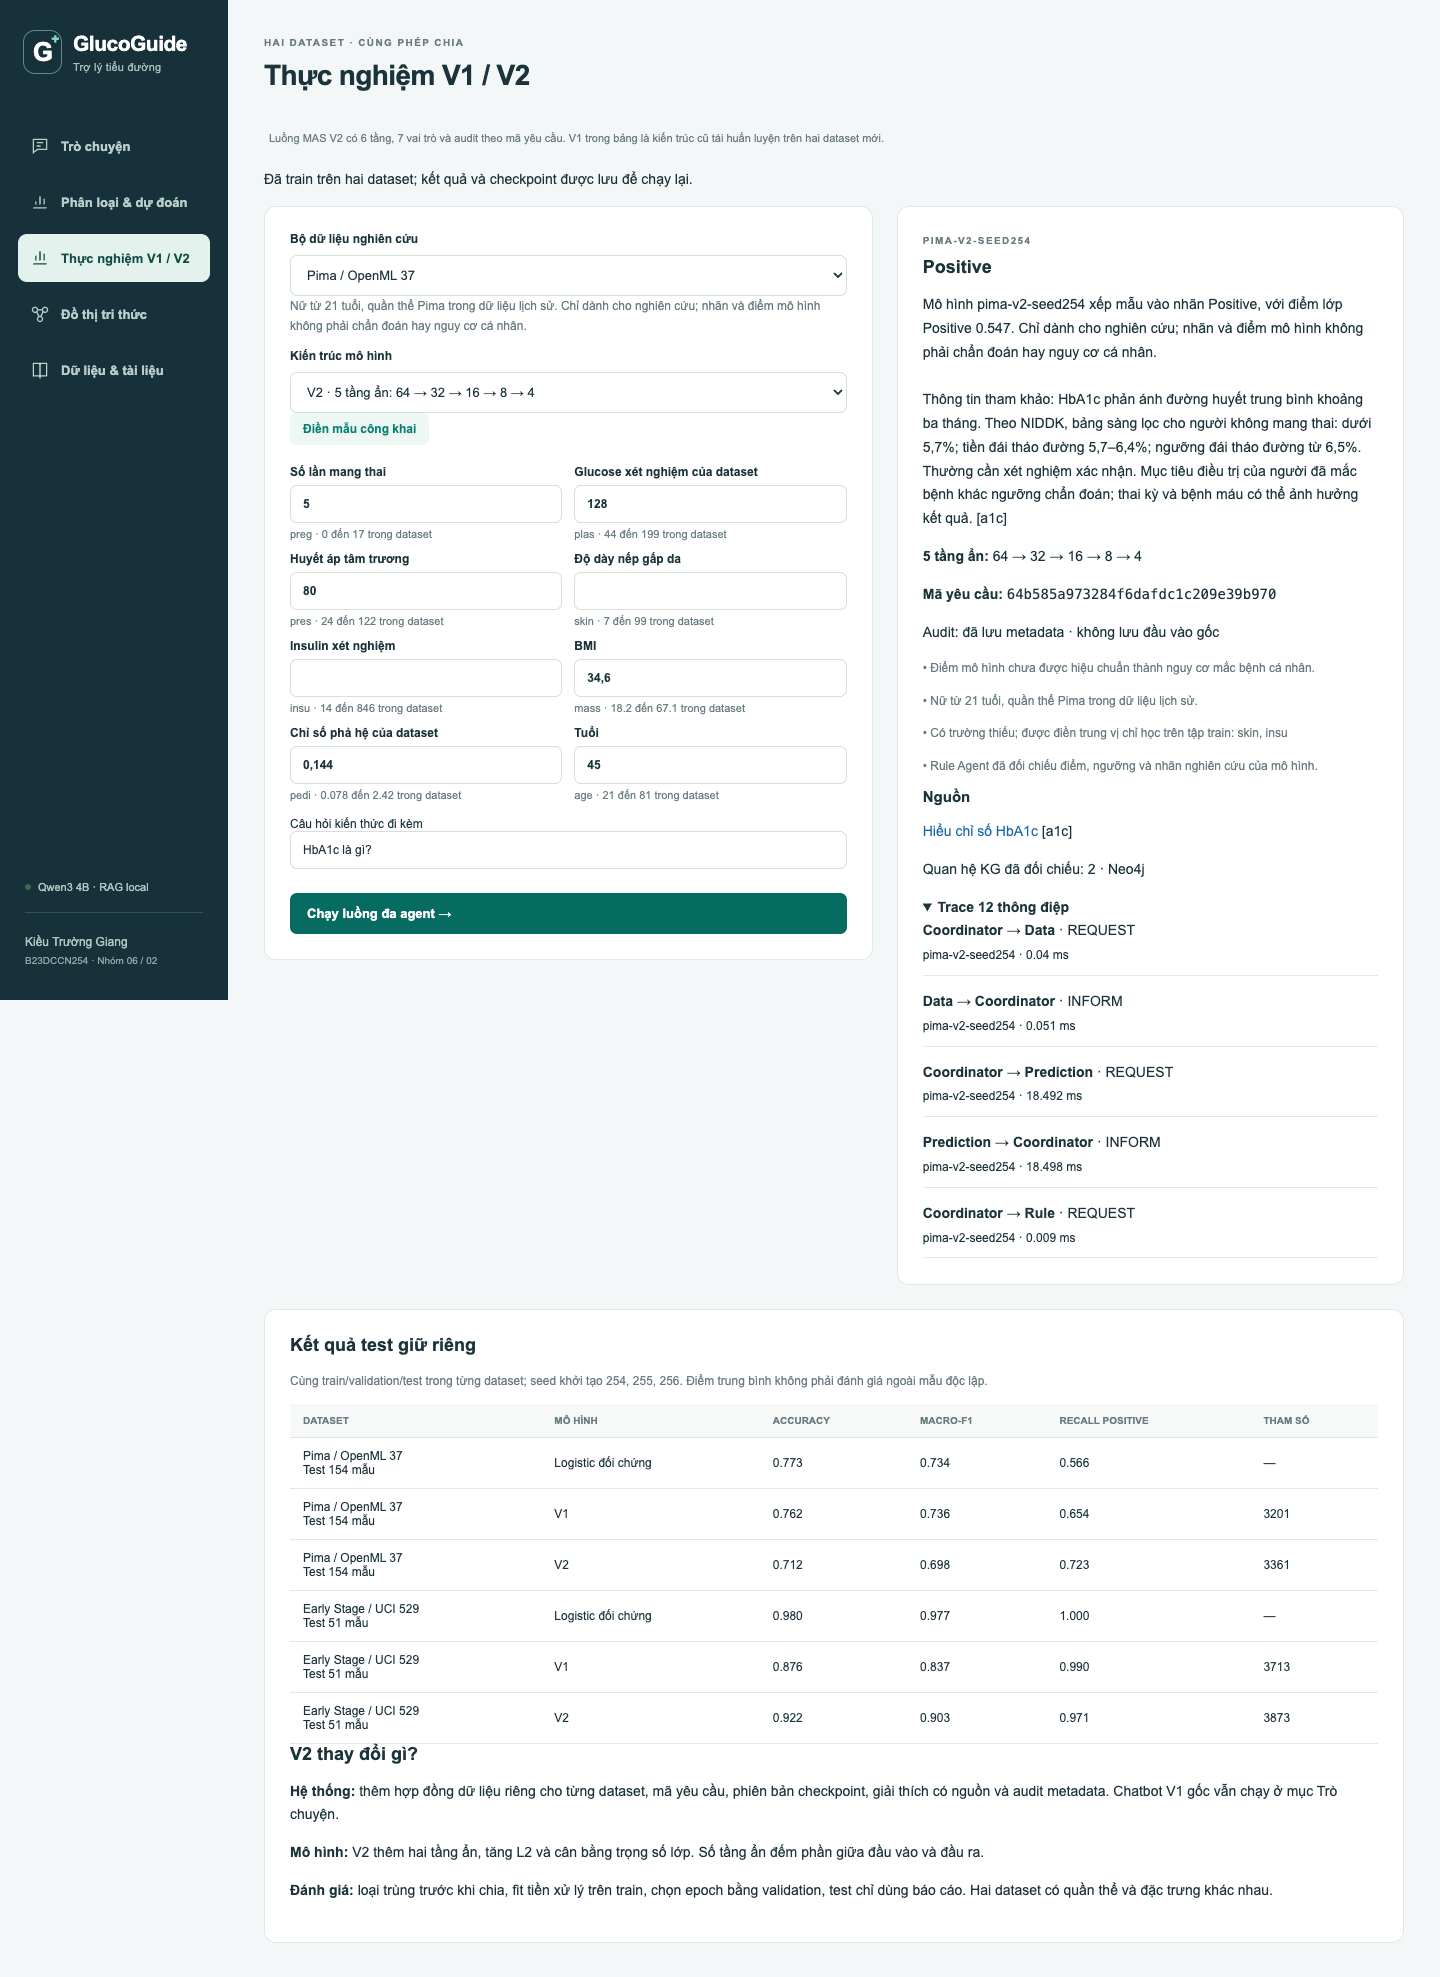
\includegraphics[width=\linewidth,height=0.72\textheight,keepaspectratio]{figures/demo-v2.png}\caption{Ảnh thật màn thực nghiệm V1/V2 trên Mac: form Pima, kết quả, nguồn, audit và bảng metric.}\end{figure}
Chọn Pima, điền mẫu công khai và chạy V2. Trace thể hiện Coordinator gửi Data và nhận feature order/missing flags; Prediction trả nhãn và hash; Rule trả cờ; KG/RAG trả đoạn và cạnh; Explanation trả nội dung có nguồn; Monitoring xác nhận lưu metadata. Request ID trên giao diện dùng đối chiếu với dòng JSONL. Không giải thích hash là bằng chứng độ đúng y khoa: hash chỉ nhận diện đúng artifact.

Nếu đổi sang V1 đối chứng, model version và hidden layers thay đổi; cùng feature và dataset vẫn được dùng. Thay dataset thì form/schema thay đổi, không giữ các số của Pima để đưa sang Early Stage. Lần so sánh không phải khuyến nghị thay thuốc hoặc thay cách điều trị.

\section{Giới hạn còn lại}
Hai bộ nhỏ, một phép chia cố định, ba khởi tạo và dữ liệu lịch sử chưa cho đánh giá ngoài phân phối. Điểm model chưa calibration; chưa có đánh giá bác sĩ. TF-IDF có thể yếu với paraphrase ngoài kho; graph phân mảnh và không suy luận nhiều bước. Verifier Qwen là bộ lọc kỹ thuật hữu hạn. Audit local chưa có phân quyền, retention hoặc dashboard quản trị; bản demo giới hạn ở loopback trên laptop.

\section{Đánh giá theo tầng và đọc thời gian chạy}
\par\FloatBarrier\begin{table}[H]\centering\small\setstretch{1.15}\setlength{\tabcolsep}{5pt}
\caption{Bốn lượt kiểm tra API V2, thời gian tới trước bước ghi audit.}\begin{tabular}{lrrr}\toprule
Model / phiên bản & Thời gian (ms) & Thông điệp & Cạnh đã đối chiếu\\\midrule
pima-v1-seed254 & 146.9 & 12 & 2\\
pima-v2-seed254 & 9.1 & 12 & 2\\
early\_stage-v1-seed254 & 10.3 & 12 & 2\\
early\_stage-v2-seed254 & 7.6 & 12 & 2\\\bottomrule\end{tabular}\end{table}

Mỗi tổ hợp trong bảng chạy một lần. \code{seconds} đo từ khi Coordinator nhận lượt tới trước Monitoring. \code{elapsed_ms} đo mỗi lời gọi MessageBus, lặp trên thông điệp yêu cầu và kết quả. Chỉ lấy một giá trị cho mỗi lời gọi. Bảng minh họa độ trễ của API thực nghiệm, chưa đo Qwen, độ trễ trình duyệt hay tải đồng thời.

Hit@4 đo nguồn kỳ vọng có xuất hiện trong bốn kết quả đầu. Để chấm câu trả lời, cần đối chiếu từng ý với nguồn và thử ca thiếu hoặc mâu thuẫn căn cứ. Bảng kiểm thử chứng minh các ca phần mềm đã chạy. Chất lượng lâm sàng cần đánh giá chuyên môn.

\chapter{Minh chứng demo V2}\label{pr:walkthrough}
\section{Giữ nguyên mẫu Pima và đổi phiên bản}
Mở mục \emph{Thực nghiệm V1/V2}, chọn Pima, điền mẫu công khai và giữ câu hỏi HbA1c. Chạy lần lượt V1 đối chứng rồi V2. Hai ảnh dưới đây được chụp từ hai lượt gọi API thành công trên Mac, với cùng vector. V1 có ba lớp ẩn và điểm Positive 0,5239. V2 có năm lớp ẩn và điểm 0,5472. Cả hai điểm qua ngưỡng 0,5. Đây là ví dụ cho thấy có thể đổi điểm mà giữ nguyên nhãn.

Khi giải thích, chỉ lần lượt mã checkpoint, số lớp, điểm, ngưỡng, nguồn và trạng thái audit. Hai lượt có mã yêu cầu khác nhau. Các mã, điểm đầy đủ và SHA-256 của checkpoint được lưu trong \nolinkurl{results/v2/project_visual_evidence.json}. Đây là chứng cứ ở cấp một lượt chạy. Để nói về kết quả tổng quát, mở bảng test và bảng đổi trạng thái ở Chương~\ref{pr:model}.

\begin{figure}[H]\centering
\begin{minipage}[t]{.48\linewidth}\centering
\textbf{V1 đối chứng}\par\smallskip
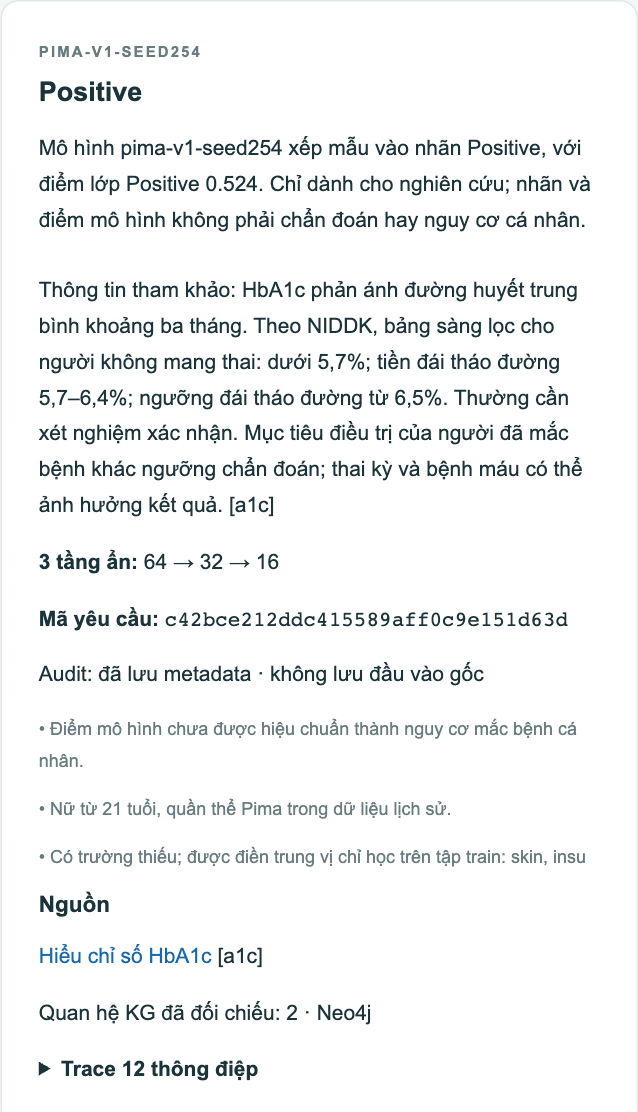
\includegraphics[width=\linewidth,height=.43\textheight,keepaspectratio]{figures/pima-v1-result.png}
\end{minipage}\hfill
\begin{minipage}[t]{.48\linewidth}\centering
\textbf{V2}\par\smallskip
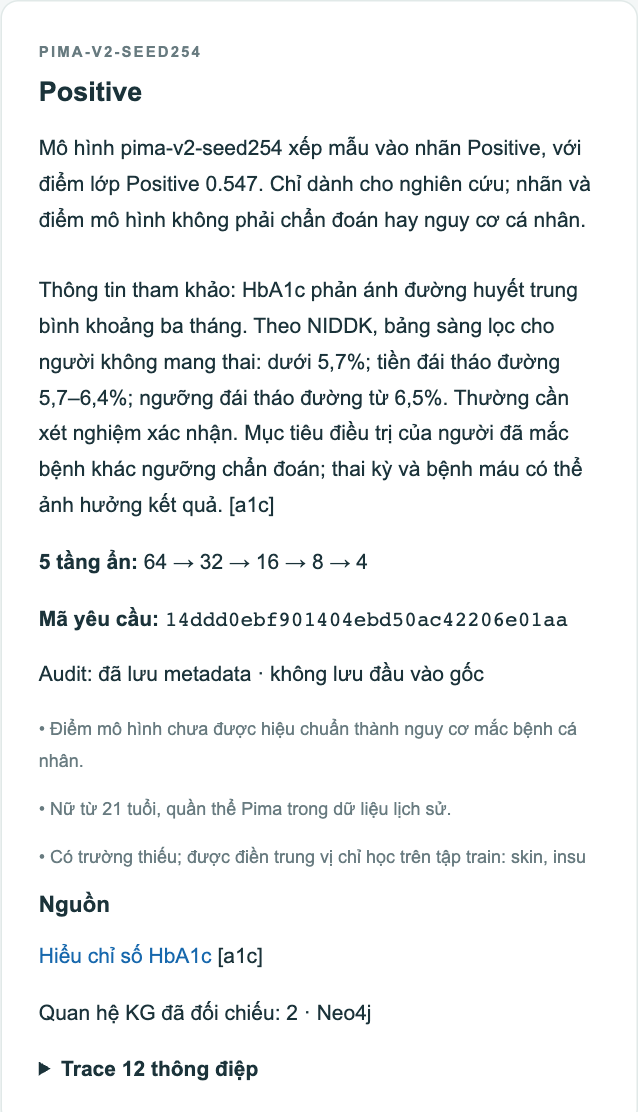
\includegraphics[width=\linewidth,height=.43\textheight,keepaspectratio]{figures/pima-v2-result.png}
\end{minipage}
\caption{Hai phản hồi thật trên cùng mẫu Pima. Mỗi lượt có mã yêu cầu, cấu hình mạng và nguồn a1c.}
\label{fig:paired-pima-ui}
\end{figure}
\FloatBarrier

\section{Từ nguồn a1c sang đồ thị Neo4j}
Mở mục \emph{Đồ thị tri thức} và chọn HbA1c trong danh sách chủ đề. Đồ thị con có ba nút và hai cạnh. Chọn nút HbA1c để thấy hai chiều quan hệ đi vào và đi ra. Dùng mã \code{a1c} trong phản hồi để đối chiếu trường \code{document} của cạnh. Sau đó có thể chuyển sang Neo4j Browser để chạy truy vấn ở Chương~\ref{pr:knowledge}.

\begin{figure}[H]\centering
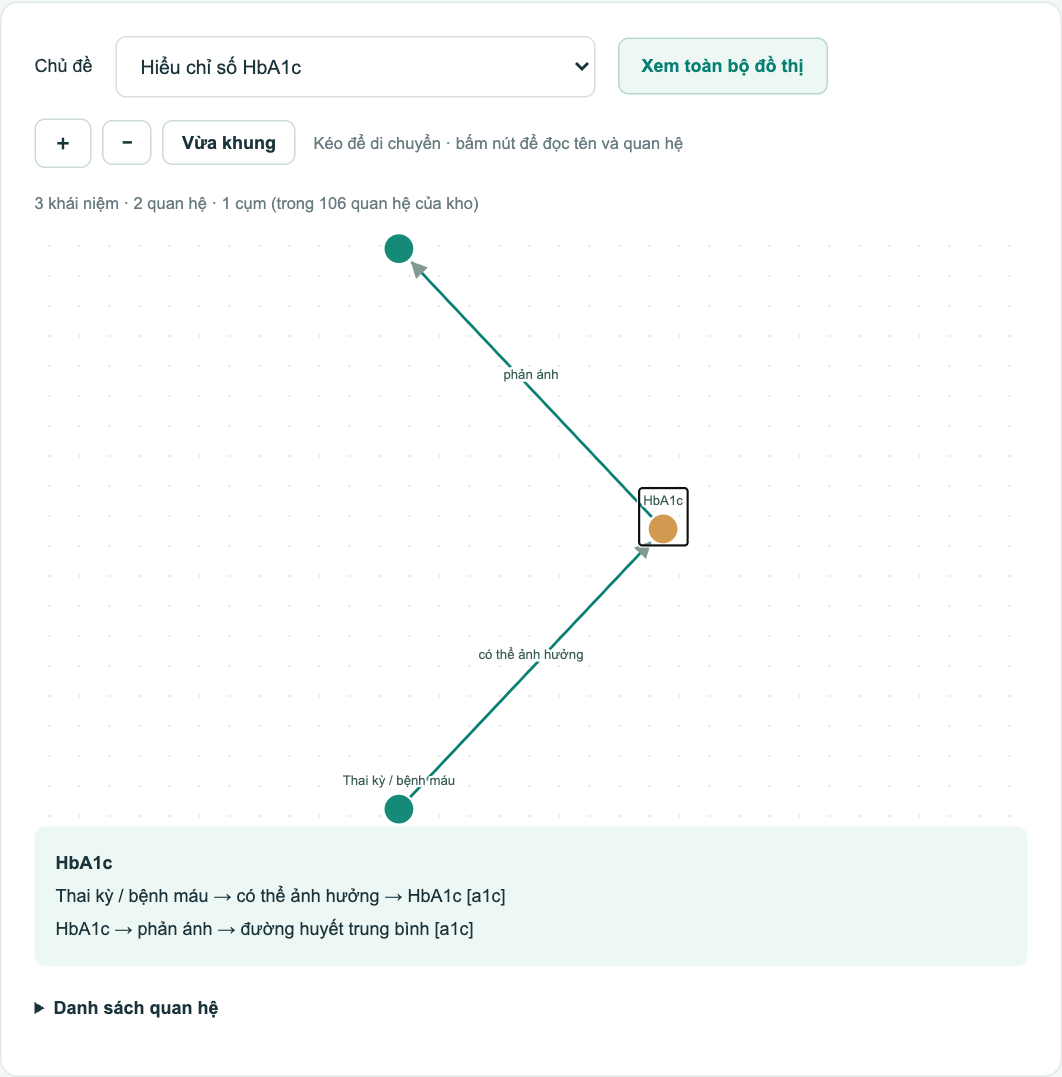
\includegraphics[width=.86\linewidth,height=.45\textheight,keepaspectratio]{figures/neo4j-a1c-live.png}
\caption{Đồ thị a1c lấy từ Neo4j đang chạy. Nút được chọn hiển thị hai cạnh đi vào và đi ra.}
\label{fig:a1c-live}
\end{figure}
\FloatBarrier

Neo4j trả quan hệ theo mã tài liệu và hệ thống so lại với đoạn nguồn. Khi trình bày, chỉ hướng cạnh và mở văn bản kèm URL để đối chiếu. Nhánh MLP xử lý vector Pima qua checkpoint riêng.

\section{Hỏi kiến thức trong luồng Trò chuyện}
Lượt chụp sau dùng câu hỏi về cách chia một bữa ăn. Phản hồi báo chế độ \code{qwen4-rag}, dùng nguồn \code{plate} và có ngữ cảnh Neo4j. Cột nguồn bên phải cho phép kiểm tra đoạn căn cứ. Bước sinh và bước đối chiếu tài liệu phục vụ việc giải thích bằng văn bản.

\begin{figure}[htbp]\centering
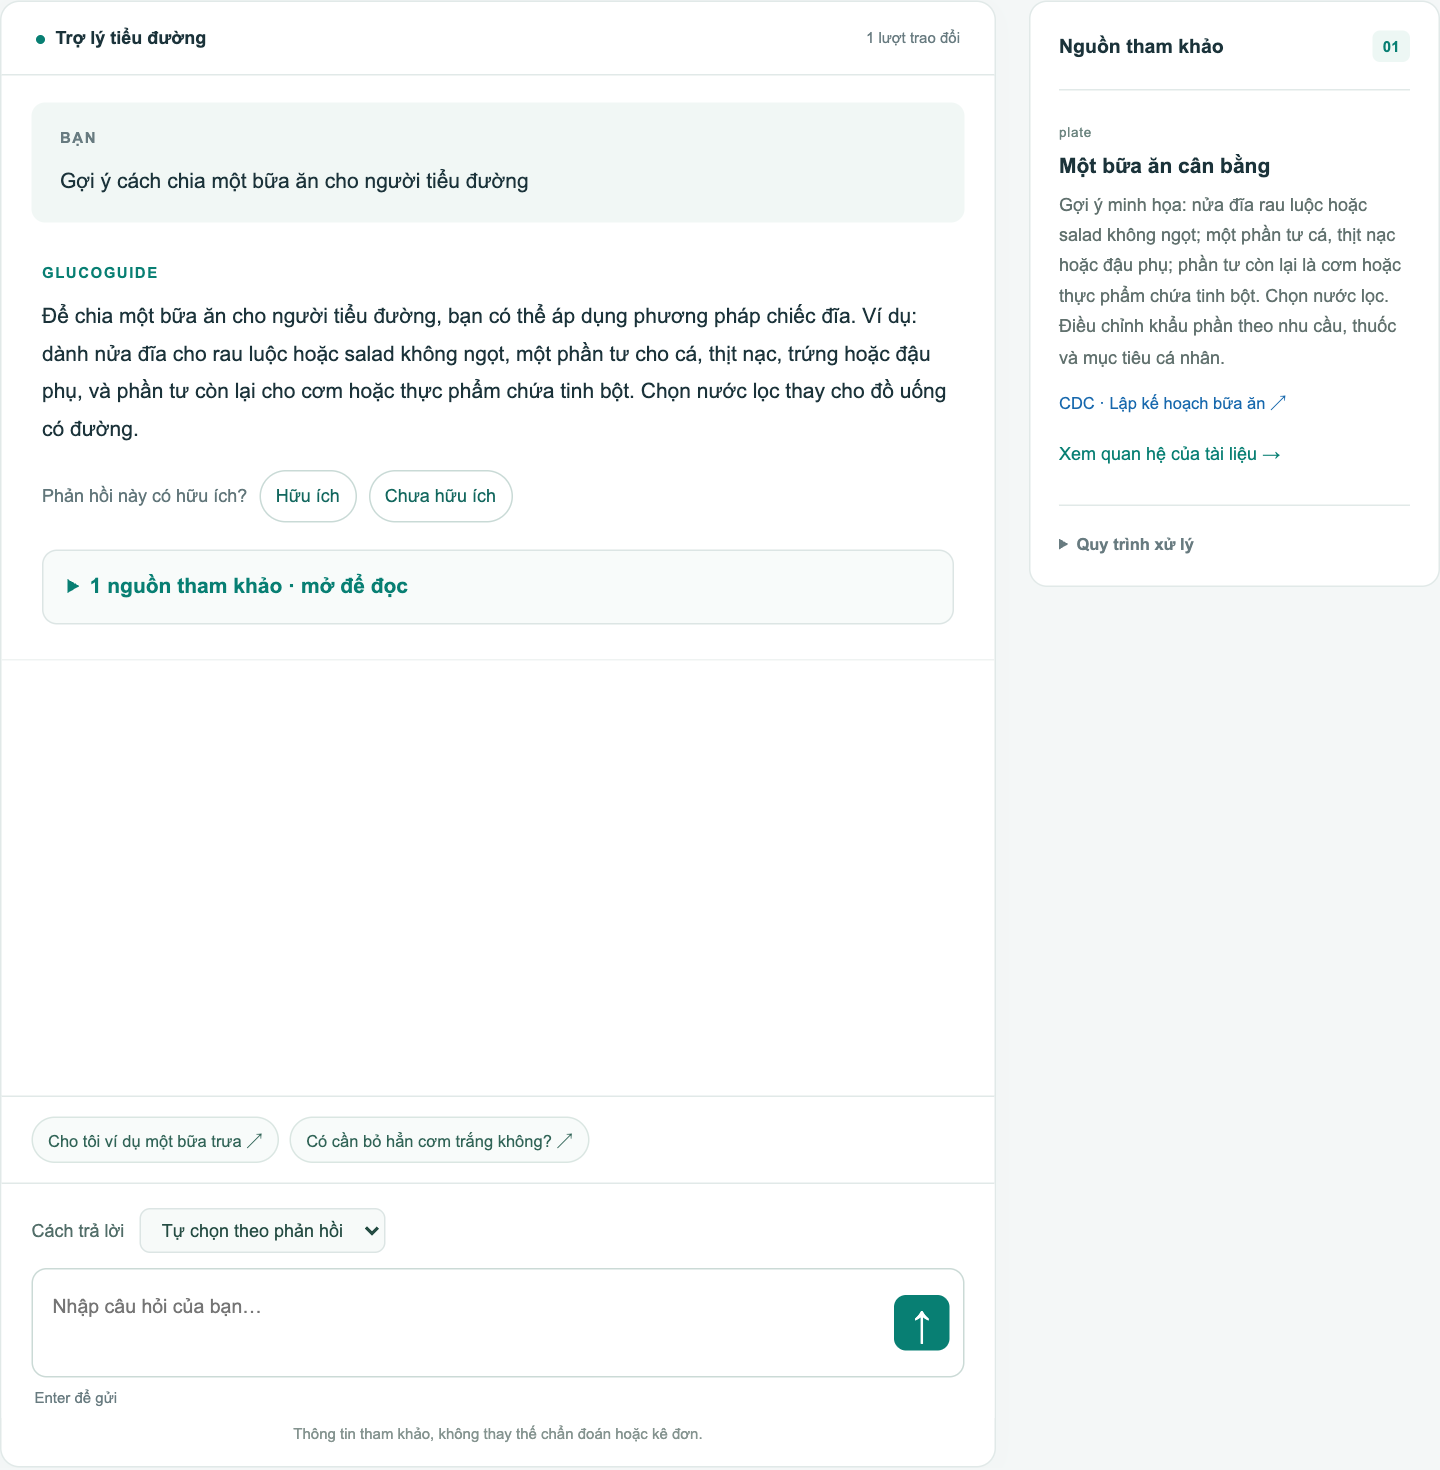
\includegraphics[width=\linewidth,trim=0 800bp 0 0,clip]{figures/chat-live-sources.png}
\caption{Một lượt Trò chuyện trên Mac. Giao diện hiển thị câu trả lời cùng nguồn truy xuất đã dùng.}
\label{fig:chat-live}
\end{figure}
\FloatBarrier

Luồng thực nghiệm dùng Explanation dạng mẫu. Luồng Trò chuyện dùng Qwen khi đủ điều kiện và chuyển sang phản hồi KB khi câu hỏi thuộc nhánh bảo vệ hoặc bản sinh không qua kiểm chứng.

\section{Điểm khác phiên bản và bằng chứng để mở}
\begin{enumerate}
\item \textbf{Model thay đổi gì?} Mở ảnh cặp ở Hình~\ref{fig:paired-pima-ui}, chỉ ba lớp và năm lớp. Sau đó mở bảng test để nêu mức tăng macro-F1 trên Early Stage và mức giảm trên Pima.
\item \textbf{Hệ thống thay đổi gì?} Mở trace ở màn thực nghiệm. Chỉ Data trước Prediction và phần Monitoring ở cuối. Trình bày vai trò của mã lượt, phiên bản model và hash.
\item \textbf{Nguồn có thực sự đi từ Neo4j hay không?} Mở Hình~\ref{fig:a1c-live}, lọc mã đoạn rồi đối chiếu JSON. Mở \code{kb_diabet.cypher} để chỉ các dòng chứa quan hệ và lệnh MERGE.
\item \textbf{Qwen có phải model phân loại?} Mở Hình~\ref{fig:chat-live} để chỉ vai trò sinh câu trả lời. Mở phần Prediction và checkpoint trong Chương~\ref{pr:mas} để giải thích phép phân lớp.
\end{enumerate}

\chapter{Chạy, trình bày và bộ nộp gọn}
\section{Khởi chạy trên Mac}
Môi trường Python nằm trong \code{.venv/} của project, không cài gói vào Miniforge base. Runtime nằm trong \code{.runtime/}, Qwen trong \code{.local-models/}. Các thư mục này và credential được loại khỏi gói code. Trên máy đã setup:
\begin{quote}\ttfamily bash run-macos.sh start\\bash run-macos.sh status\\bash run-macos.sh stop\end{quote}
Mở \url{http://localhost:8765}. Qwen dùng cổng 11435; Neo4j Bolt 7687 và Browser 7474. Launcher có restart để nạp code mới. Người khác không thể dùng localhost của họ để truy cập laptop này. Bản \url{https://glucoguide-giang254.vercel.app/} chạy MLP và truy xuất KB. Khi Aura mất kết nối, nó trả bản chụp có nhãn. Qwen qua llama.cpp và audit lưu tệp thuộc môi trường Mac.

Máy khác cần Python 3.14 và Java 21 ARM64; chạy setup-macos, setup-v2-assets nếu cần tải lại nguyên liệu train, train-v2 nếu chủ động tạo lại checkpoint, rồi start. Các checkpoint V2 và CSV sạch có trong gói nên không cần train lại chỉ để demo. Tệp dữ liệu nén Diabetes 50K cũ chưa khôi phục do endpoint Kaggle trả 404; việc này không chặn inference các model đã có hoặc hai thực nghiệm mới.

\section{Kịch bản thuyết trình khoảng bảy phút}
\begin{enumerate}
\item Phút 0--1: bài toán, giới hạn nghiên cứu và bảng V1/V2; nêu ba thay đổi thật.
\item Phút 1--2: trình bày sáu tầng hệ thống, bảy vai trò agent và năm tầng ẩn MLP V2.
\item Phút 2--3: hai dataset, loại trùng, chia 60/20/20; đọc kết quả và một đánh đổi.
\item Phút 3--4: chạy mẫu công khai V2 và mở trace/request ID.
\item Phút 4--5: hỏi chat, mở nguồn; xem Neo4j và file Cypher.
\item Phút 5--6: PDF nguồn và đường đi KB--RAG--KG; nêu TF-IDF chứ không neural embedding.
\item Phút 6--7: trình bày kết quả kiểm thử, giới hạn và hướng phát triển.
\end{enumerate}

\section{Thư mục bàn giao và đường dẫn trên GitHub}
Mã nguồn và báo cáo được lưu tại \url{https://github.com/jellalaz/He_Thong_Thong_Minh_Thay_Que}. Mở trực tiếp \href{https://github.com/jellalaz/He_Thong_Thong_Minh_Thay_Que/tree/main/exports/KB_KG_RAG}{thư mục KB, KG và RAG} để xem tệp Cypher và các tệp tri thức.

Hai PDF V2 nằm trong \code{reports/}. Mở \nolinkurl{exports/KB_KG_RAG/} để xem trực tiếp mười tệp tri thức, gồm \code{kb_diabet.cypher}. Bản gom trên Mac đặt mã nguồn trong \code{MA_NGUON/} và hướng dẫn trong \code{DOC_TRUOC.txt}.

\section{Hướng phát triển có thứ tự}
Ưu tiên đánh giá ngoài mẫu và chất lượng nguồn trước khi tăng độ sâu mạng. Sau đó có thể hiệu chuẩn xác suất trên validation độc lập, kiểm tra nhiều phép chia theo người/bệnh viện, bổ sung kiểm thử paraphrase, đánh giá câu trả lời bởi người có chuyên môn và quản lý audit. Nếu triển khai semantic retrieval hoặc multi-hop KG, cần benchmark mới và version mới; không mô tả các đề xuất đó như phần đã chạy của V2.
